

Im \Abschnitt\ref{cha:2_sub_Begriff_der_Schirmdaempfung} wurde bereits auf den Begriff der Schirmdämpfung als Pegelmaß der Feldgrößen\-beträge (vgl. \Gleichungen\eqref{eq:2_Schirmdaempfung_elektrisch} bis \eqref{eq:2_Schirmdaempfung_Leistung}) eingegangen. Bei der Bestimmung der Schirmdämpfung mit einem VNA eignet sich jedoch die Betrachtung der Messstrecke mithilfe der Zweitortheorie. Dabei stellt diese einen passiven Zweipol dar, der sich analog zu einem passiven elektrischen Bauelement verhält und durch Wellengrößen eindeutig beschrieben werden kann. In der \Abb\ref{fig:4_Zweitor} ist dies schematisch dargestellt, wobei die jeweils zulaufenden Wellen durch die Größen $\underline{a}_1$ und $\underline{a}_2$ und die ablaufenden mit $\underline{b}_1$ und $\underline{b}_2$ gekennzeichnet sind~\cite{Taschenbuch_HF-Technik}. 
\par
\vspace{\linespace}


\begin{figure}[ht]
    \centering
    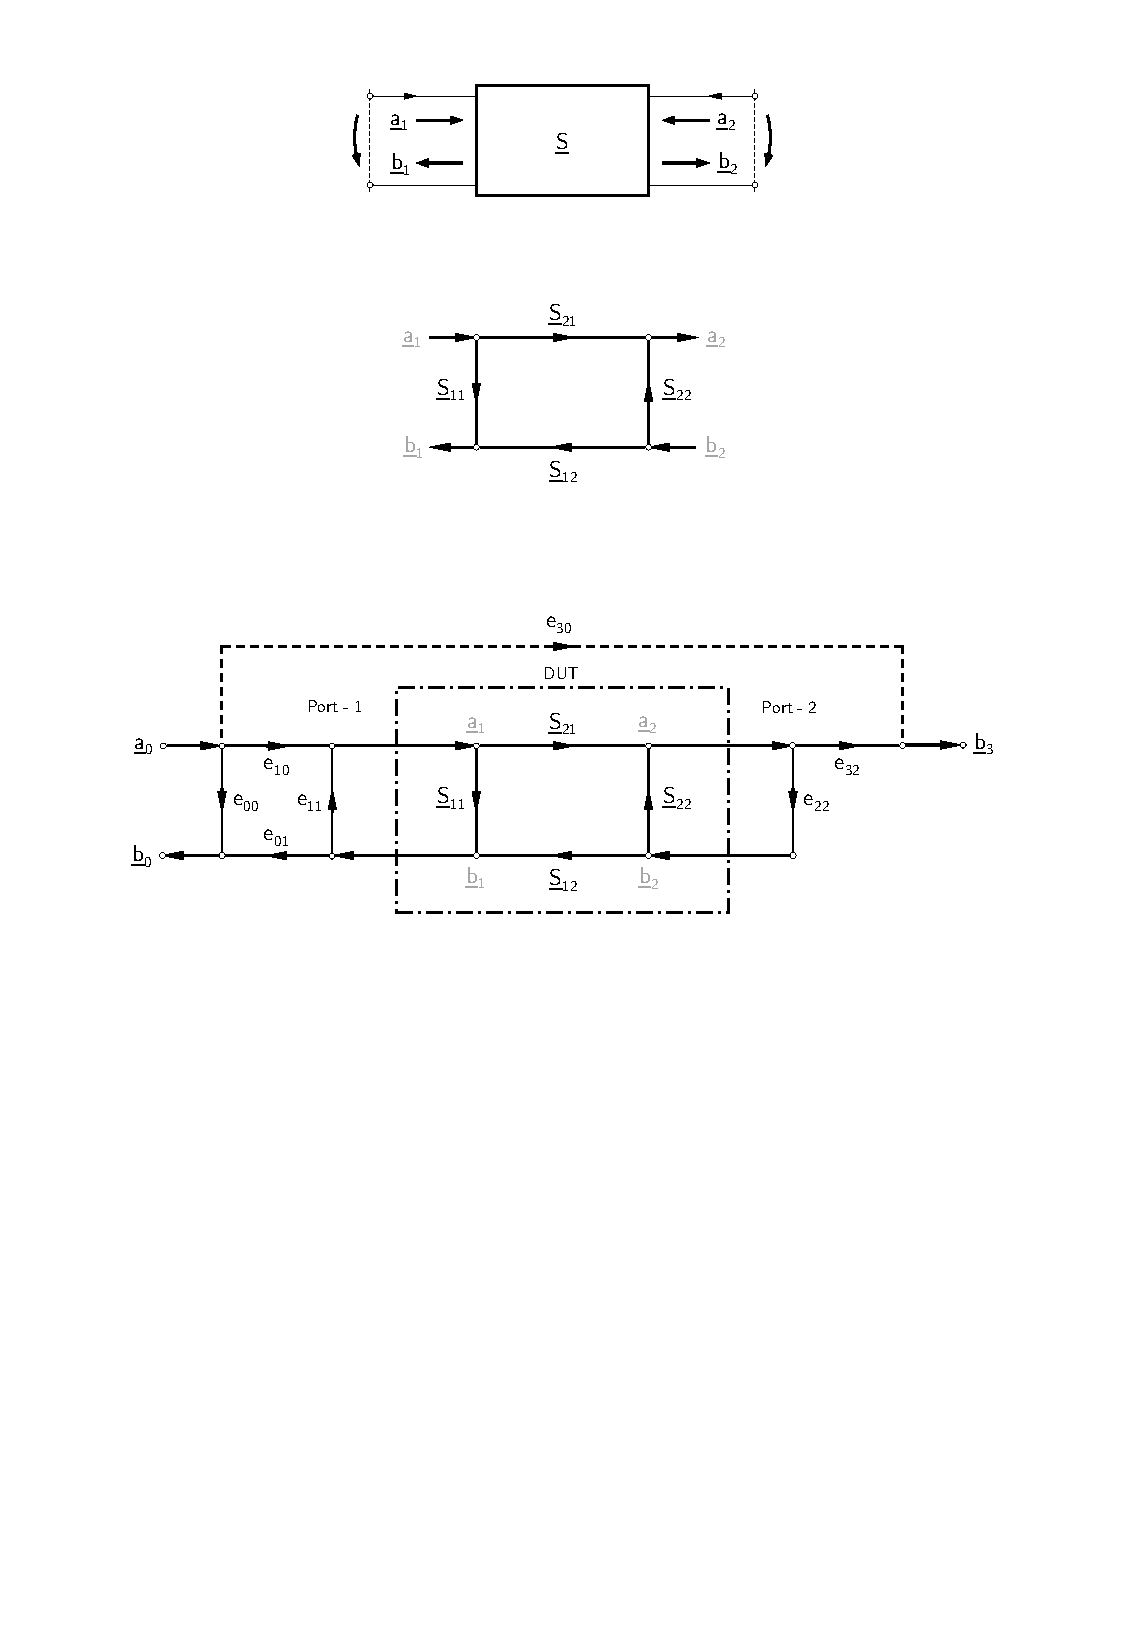
\includegraphics[page = 1, trim = 5.9cm 24cm 5.9cm 1.3cm, clip, width = 0.5\textwidth]{Abbildungen/Kapitel4/Zweitor.pdf}
    \caption[Zweitor mit Wellengrößen]{Zweitor mit Wellengrößen nach~\cite{Taschenbuch_HF-Technik}}
    \label{fig:4_Zweitor}
\end{figure}


In der Praxis hat die Darstellung mithilfe der Wellengrößen den Vorteil, dass diese auch bei hohen \mbox{Frequenzen} direkt gemessen werden können~\cite{Taschenbuch_HF-Technik}. Neben der äquivalenten Beschreibung des Verhaltens des Zweitors durch Beziehungen zwischen den Torspannungen und -strömen, kann das Übertragungsverhalten auch mithilfe der Streumatrix $\underline{S}$ 


\begin{equation}
\centering
    \left(\begin{array}{c}\underline{b}_1 \\ \underline{b}_2 \end{array}\right) = \left(\begin{array}{cc}\underline{S}_{11} & \underline{S}_{12} \\ \underline{S}_{21} & \underline{S}_{22} \end{array}\right) \left(\begin{array}{c}\underline{a}_{1} \\ \underline{a}_{2} \end{array}\right) \label{cha:4_Streuparameter}
\end{equation}

charakterisiert werden~\cite{Taschenbuch_HF-Technik}. $\underline{S}$ ist für struktursymmetrische Zweitore ebenfalls symmetrisch~\cite{Grundkurs_Hochfrequenztechnik}.  
\par
\vspace{\linespace}
Die Bestimmung der Streuparameter oder S-Parameter $\underline{S}_{11}$ bis $\underline{S}_{22}$ kann nun durch die Beschaltung jeweils eines Tores mit der Systemimpedanz durch den VNA erfolgen. Dies führt im Idealfall zum reflexionsfreien Abschluss des Tores, wodurch die jeweils zulaufende Wellengröße $\underline{a}_1$ bzw. $\underline{a}_2$ verschwindet~\cite{Grundkurs_Hochfrequenztechnik}. Die Berechnung der Streuparameter mithilfe der \Gleichung\eqref{cha:4_Streuparameter} wird damit trivial. 
\par
\vspace{\linespace}
Für die Deutung der S-Parameter ist die Reihenfolge der Indizes relevant. $\underline{S}_{11}$ und $\underline{S}_{22}$ beschreiben den primären bzw. sekundären Reflektionsfaktor bei Abschluss des jeweils anderen Tores. Der Transmissionskoeffizient $\underline{S}_{21}$ charakterisiert die Transmission von 1 nach 2 bei abgeschlossenem Tor 2. Die Bedeutung von $\underline{S}_{12}$ ergibt sich analog durch Vertauschen der Tore. Das Signalflussdiagramm in \Abb\ref{fig:4_Signalflussdiagramm_Zweitor} veranschaulicht die Zuordnung der Indizes zu den einzelnen Streuparametern.
\par
\vspace{\linespace}

\begin{figure}[ht]
    \centering
    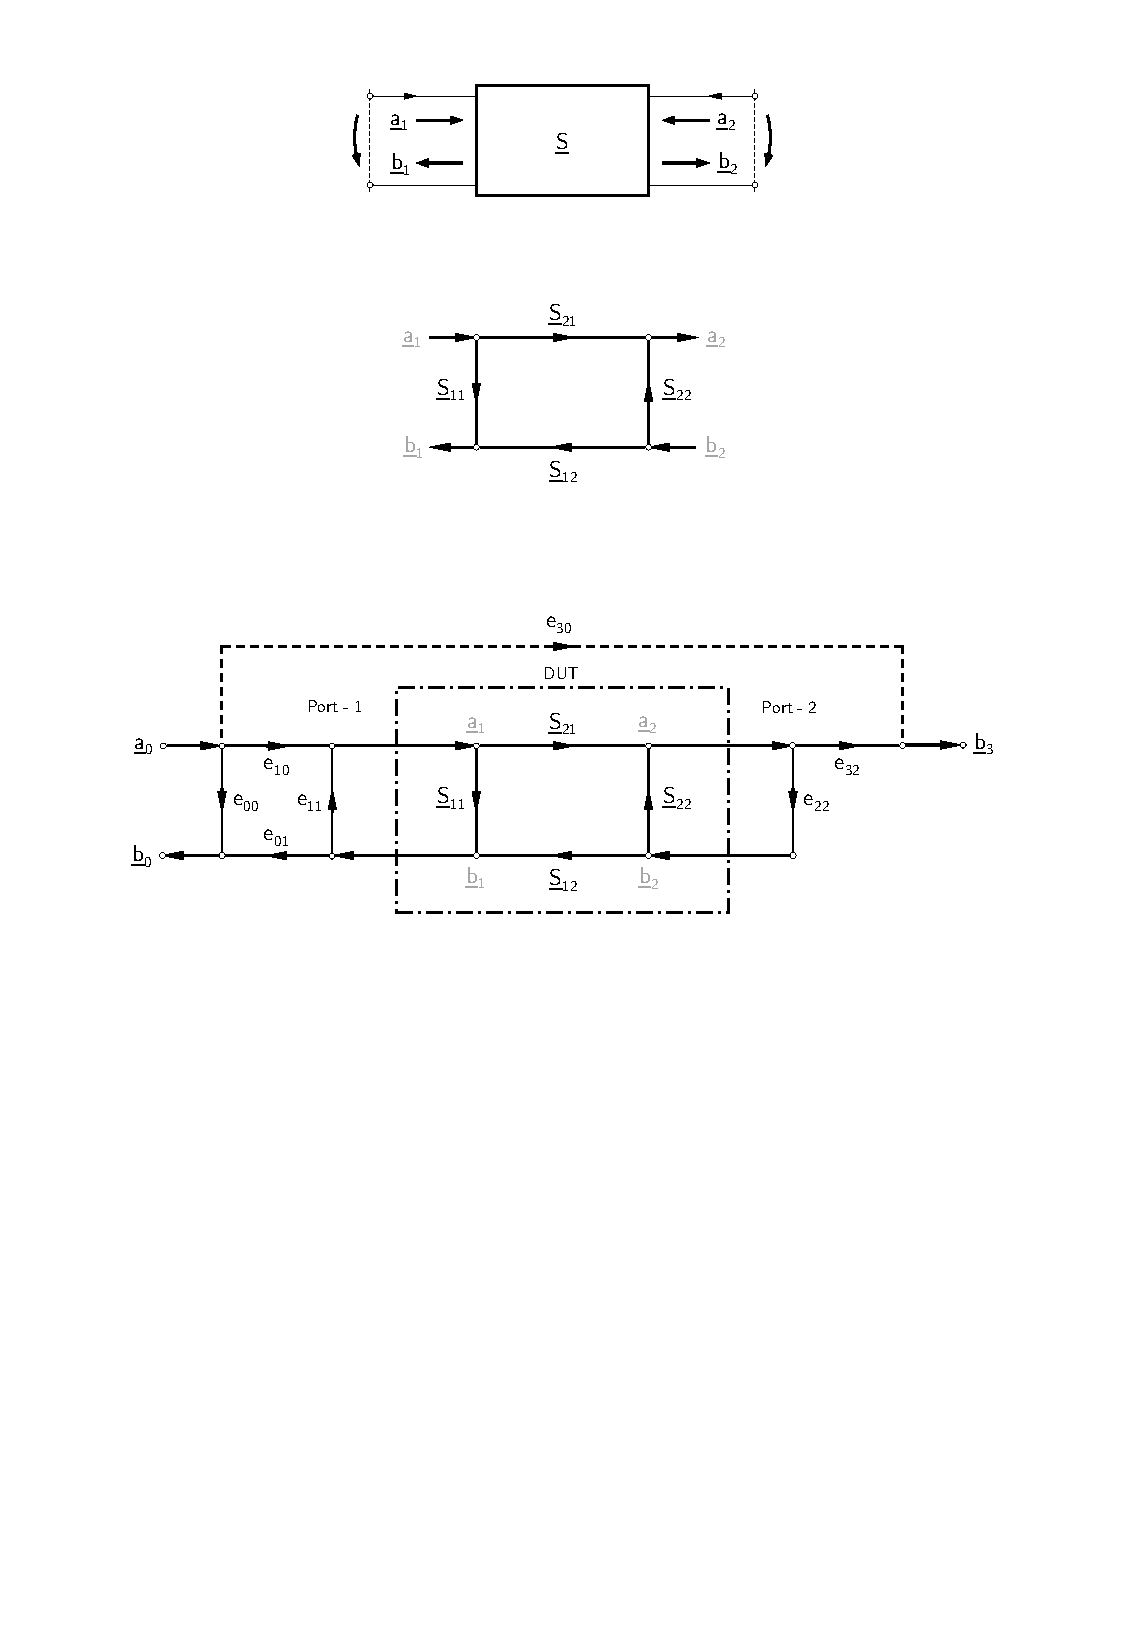
\includegraphics[page = 1, trim = 5.9cm 19.2cm 5.9cm 5cm, clip, width = 0.5\textwidth]{Abbildungen/Kapitel4/Zweitor.pdf}
    \caption[Signalflussdiagramm eines Zweitors mit Streuparametern]{Signalflussdiagramm eines Zweitors mit Streuparametern nach~\cite{Grundkurs_Hochfrequenztechnik}}
    \label{fig:4_Signalflussdiagramm_Zweitor}
\end{figure}

Um mit der ermittelten und im Allgemeinen komplexen Streumatrix als Übertragungsmaß zu arbeiten, bietet sich die logarithmische Darstellung an, weshalb die Angabe der S-Parameter oft in Dezibel erfolgt~\cite{Grundkurs_Hochfrequenztechnik} 

\begin{equation}
    S_{12, dB} = 20 \cdot \lg \left( \left| \underline{S}_{12} \right| \right) \; \text{.} \label{eq:4_Schirmdaempfung_Dezibel}
\end{equation}


Mithilfe der Transmissionskoeffizienten kann die Schirmdämpfung eines Materials durch Einfügungs\-messung ermittelt werden (vgl. \Abschnitte\ref{cha:2_sub_Begriff_der_Schirmdaempfung} und \ref{cha:2_Methoden_der_Schirmdaempfungsmessung}). In der \Abb\ref{fig:4_Einfuegungsmessung} ist die Vorgehensweise schematisch dargestellt. Beim Arbeiten mit den S-Parametern in Dezibel kann die Schirmdämpfung durch Subtraktion der ermittelten Freiraumdämpfung ohne Schirm von den Messwerten mit Schirm bestimmt werden. Dies wird für alle Frequenzen des Messbereichs durchgeführt.
\par



\begin{figure}[ht]
    \centering
    \begin{subfigure}[b]{0.99\textwidth}
        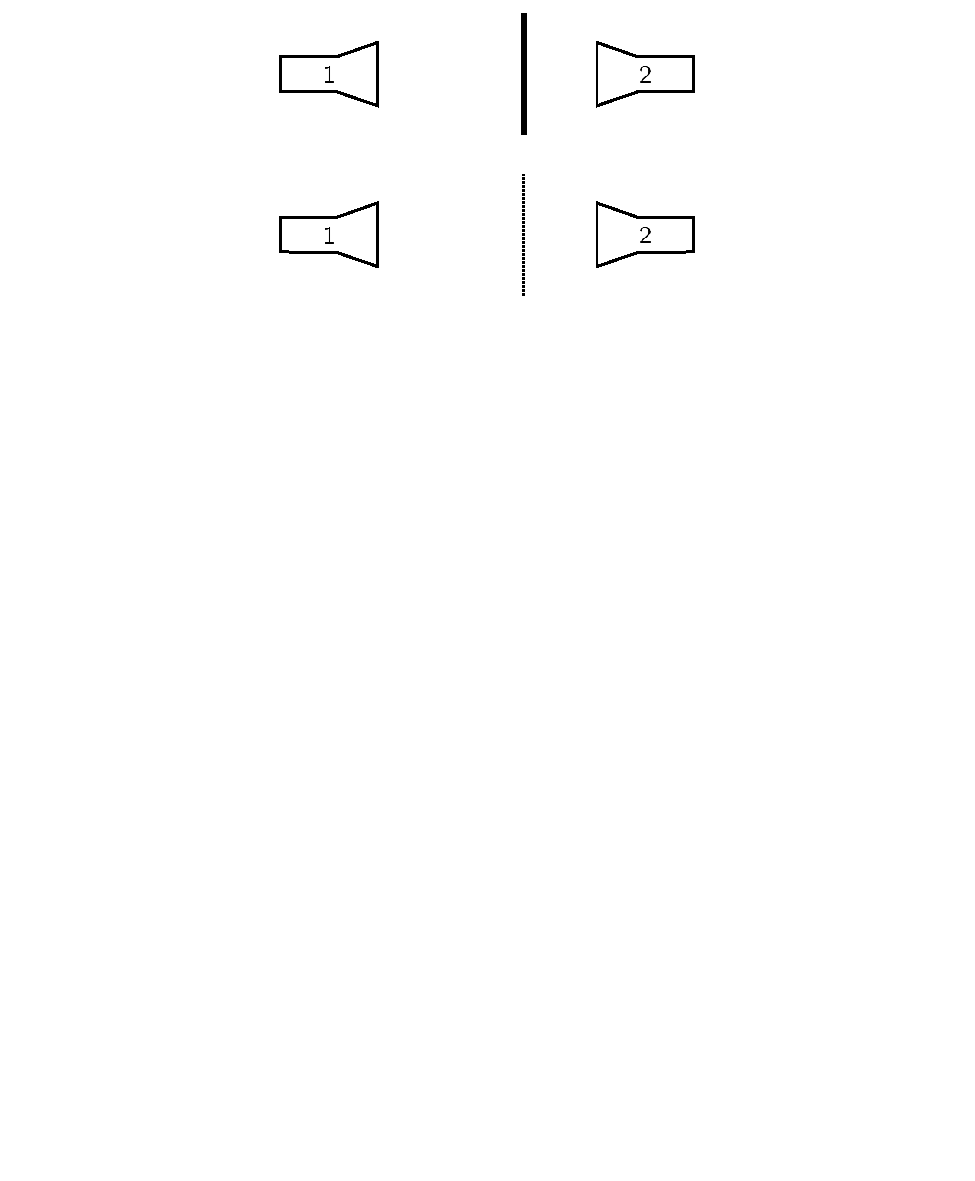
\includegraphics[page = 1, width=\textwidth, trim = 0cm 14.75cm 0cm 2.5cm, clip]{Abbildungen/Kapitel4/Einfuegungsmessung.pdf}
        \caption{\label{subfig:4_Einfuegungsmessung_Fall1}}
    \end{subfigure}
    \vspace{0.5cm}
    \begin{subfigure}[b]{0.99\textwidth}
       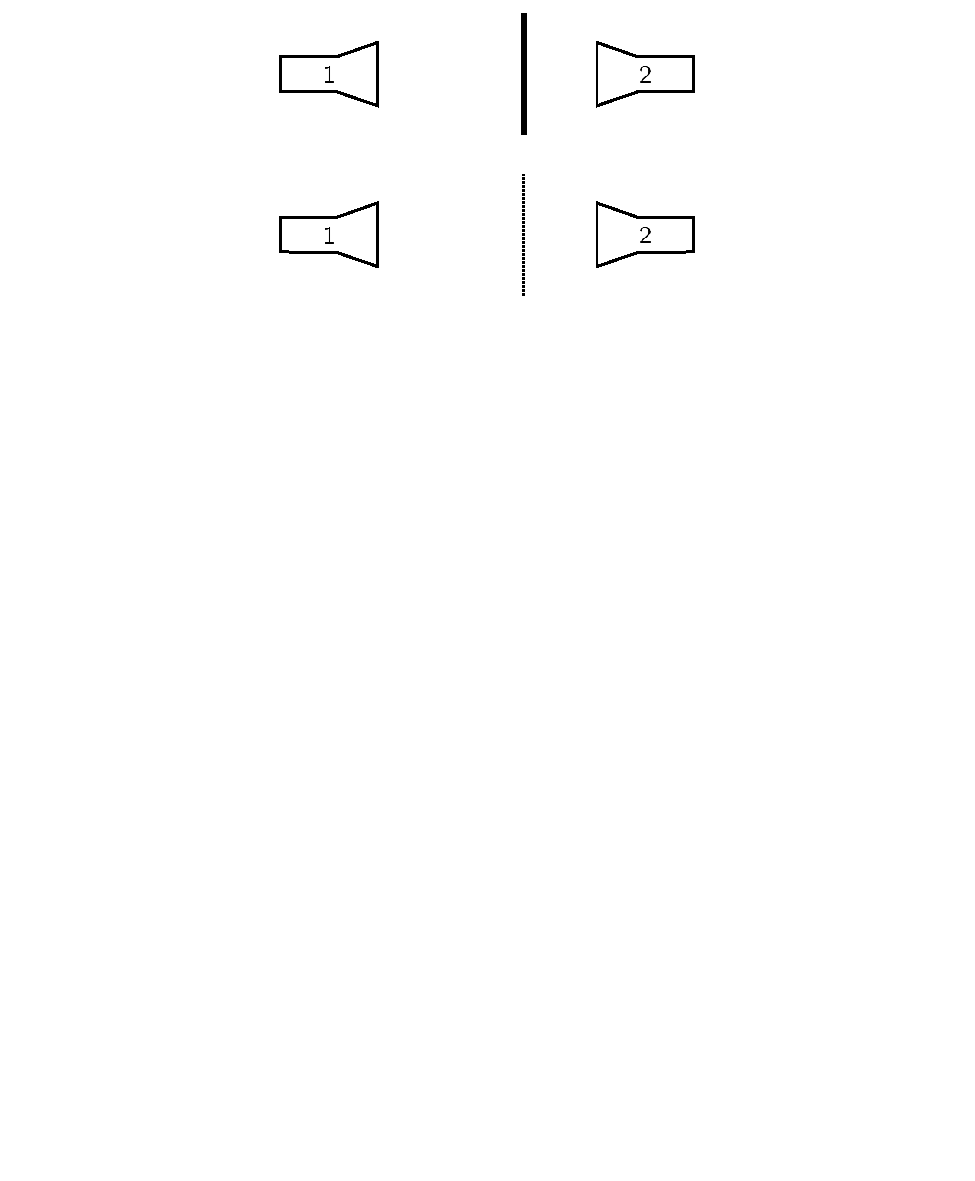
\includegraphics[page = 1, width=\textwidth, trim = 0cm 17.5cm 0cm 0cm, clip]{Abbildungen/Kapitel4/Einfuegungsmessung.pdf}
        \caption{\label{subfig:4_Einfuegungsmessung_Fall2}}
    \end{subfigure}
    \caption[Schematische Darstellung der durchgeführten Einfügungsmessung]{Schematische Darstellung der durchgeführten Einfügungsmessung im Fernfeld ohne~(\subref{subfig:4_Einfuegungsmessung_Fall1}) und mit~(\subref{subfig:4_Einfuegungsmessung_Fall2}) Schirm im Koppelpfad}
    \label{fig:4_Einfuegungsmessung}
\end{figure}


Da es sich bei den verwendeten Schirmen um rein passive Elemente handelt und im Idealfall das Reziprozitätsgesetz gilt (vgl. \Abschnitt\ref{cha:2_sub_Begriff_der_Schirmdaempfung}), sollten die Transmissionskoeffizienten der Streumatrix gleich sein. Da es trotz sorgfältiger Abdeckung der meisten reflektiven Flächen innerhalb der Testkammer Reflektionen und damit zusätzlichen Wellenfronten gibt, gilt 

\begin{equation}
    |S_{12}| \approx |S_{21}|\label{eq:4_Naeherung_Transmissionskoeffizienten}
\end{equation}

nur noch in Näherung~\cite{EM_Schirmung}. Im \Abschnitt\ref{cha:4_Versuchsvorbereitung_und_Durchfuehrung} wird darauf anhand der Messwerte noch einmal eingegangen.
\par
\vspace{\linespace}




%Bei Messung der Schirmdämpfung --> da rein passiv und nach Reziprozitätsgesetz sollte Streumatrix ebenfalls symmetrisch sein --> kann an Messwerten angelesen werden (ggf. Vergleich einfügen)

%Einfügungsmessung erklären mit Freiraumdämpfung, etc.


Für die durchgeführten Messungen wird ein 2-Port VNA genutzt. Damit ist die Bestimmung aller Streuparameter möglich. Der VNA gibt dabei das Testsignal aus und übernimmt gleichzeitig die Analyse und Bestimmung der Amplitude und Phase des empfangenen Signals. Auch wenn zur reinen Bestimmung der Schirmdämpfung nach \Gleichung\eqref{eq:4_Schirmdaempfung_Dezibel} das komplexe Ausgangsignal wieder auf einen skalaren Wert reduziert wird, kann mithilfe der Information über die Phasenlage des Signals eine höhere Genauigkeit erzielt werden~\cite{VNA-Handbuch}. Außerdem ermöglicht es zusätzliche Messmethoden wie Zeitbereichsmessungen und die Darstellung von Smith-Diagrammen. Letztere werden vor allem für die Auswertung der Reflektionsparameter genutzt~\cite{VNA-Handbuch}.

%2-Port VNA --> Quelle und Analyzer gleichzeitig

%Modellnummer und Messbereich


